\documentclass[11pt,letterpaper]{article}

% ===================== Paquetes =====================
\usepackage[utf8]{inputenc}
\usepackage[T1]{fontenc}
\usepackage{lmodern}
\usepackage[spanish,es-nodecimaldot,es-tabla]{babel}
\usepackage[margin=2.5cm]{geometry}
\usepackage{enumitem}
\setlist{itemsep=2pt, topsep=4pt, parsep=0pt}
\usepackage{graphicx}
\usepackage{booktabs}
\usepackage{array}
\usepackage{float}
\renewcommand{\topfraction}{0.9}
\renewcommand{\bottomfraction}{0.8}
\renewcommand{\textfraction}{0.07}
\renewcommand{\floatpagefraction}{0.85}
\setlength{\textfloatsep}{10pt plus 2pt minus 2pt}
\setlength{\floatsep}{8pt plus 2pt minus 2pt}
\setlength{\intextsep}{8pt plus 2pt minus 2pt}
\usepackage[font=small,labelfont=bf]{caption}
\setlength{\abovecaptionskip}{4pt}
\usepackage[hidelinks]{hyperref}
\usepackage{titlesec}
\titlespacing*{\section}{0pt}{12pt}{4pt}
\graphicspath{{figuras/}{../figuras/}}

\setlength{\parindent}{0pt}
\setlength{\parskip}{4pt}

% ===================== Datos del documento =====================
\newcommand{\tituloproyecto}{¿Mejoran el petróleo, las tasas de interés y el dólar global la predicción diaria de la TRM? LightGBM, CatBoost y XGBoost frente a una regresión lineal}
\newcommand{\integranteuno}{Nicolás Cárdenas Díaz}
\newcommand{\integrantedos}{María Paula Muñoz Malaver}

\begin{document}

% ===================== Portada =====================
\begin{titlepage}
\centering
\vspace*{1.5cm}

{\large Universidad Externado de Colombia\par}
{\large Machine Learning II\par}

\vspace{2.5cm}

{\Large \textbf{\tituloproyecto}\par}

\vspace{1cm}

{\large Segunda entrega --- Proyecto Integrador\par}
{\large Fase 2: datos, modelamiento y validación\par}

\vspace{2.5cm}

{\large \integranteuno \par}
{\large \integrantedos \par}

\vfill

{\large \today\par}

\end{titlepage}

% ===================== Cuerpo =====================

\section*{Introducción}

Comparamos los tres modelos de gradient boosting del artículo base \cite{articulo} ---LightGBM \cite{lightgbm}, CatBoost \cite{catboost} y XGBoost \cite{xgboost}--- con una regresión lineal que usa solo los movimientos recientes de la TRM. Cada modelo se entrena con solo la TRM y, aparte, agregando el petróleo Brent, el índice del dólar (DXY) y el diferencial de tasas Banrep--Fed. Así respondemos la pregunta de la Entrega~1: ¿estas variables mejoran la predicción diaria de la TRM y cuál algoritmo las aprovecha mejor?

\paragraph{Respuesta.} No la mejoran. Los tres boosting predicen la TRM de mañana igual que la regresión lineal, no mejor, y con las variables macro empeoran en el test. Ningún algoritmo las aprovecha; LightGBM es el que menos se perjudica. Lo único predecible es que parte del movimiento de hoy continúa mañana, porque la TRM es el promedio de las operaciones de un día. Esa relación es lineal y la regresión la captura completa. El petróleo y el dólar del día anterior se relacionan tan débilmente con la TRM del día siguiente (correlaciones de 0,06 a 0,09) que no alcanzan a reducir el error.

% -------------------------------------------------------------------------------------
\section*{7.1. Consolidación de los datos}

Usamos cinco series diarias, de diciembre de 2003 a septiembre de 2026, descargadas de las interfaces oficiales del Banco de la República \cite{banrep}, FRED \cite{fred} y Yahoo Finance \cite{yahoo-dxy} (Tabla~\ref{tab:calidad}). Son datos reales; no hubo simulación. Como las fuentes corrigen datos pasados, guardamos los archivos tal como llegaron, con huella MD5, y trabajamos sobre esa copia. La TRM se verificó contra la de la Superintendencia Financiera \cite{superfin}. No hay duplicados ni valores imposibles; los faltantes del Brent son festivos, y los cambios extremos son episodios reales (2008, 2020, 2026), así que se conservan. Tras alinear las series y calcular las variables, el conjunto final tiene 5.401 días (4.320 de desarrollo, 1 purgado y 1.080 de test), por encima de los 5.000 que exige la guía.

\begin{table}[!htbp]
\centering\footnotesize
\setlength{\tabcolsep}{4pt}
\caption{Fuentes y calidad de las series. Hueco máx.: días seguidos sin dato. Extremos: cambios de más de 5 desviaciones estándar (TPM: más de 100 pb).}
\label{tab:calidad}
\begin{tabular}{llcrrrrr}
\toprule
Serie & Fuente & Periodo & Obs. & Falt. & Dupl. & Hueco máx. & Extremos \\
\midrule
TRM & Banco de la República (SDMX) & dic 2003 -- sep 2026 & 5.412 & 0 & 0 & 6 & 10 \\
Brent & FRED, \texttt{DCOILBRENTEU} & dic 2003 -- sep 2026 & 5.684 & 268 & 0 & 9 & 15 \\
DXY & Yahoo Finance, \texttt{DX-Y.NYB} & dic 2003 -- sep 2026 & 5.756 & 0 & 0 & 5 & 4 \\
TPM & Banco de la República (SDMX) & dic 2003 -- sep 2026 & 8.339 & 0 & 0 & 1 & 2 \\
DFF & FRED, \texttt{DFF} & dic 2003 -- sep 2026 & 8.338 & 0 & 0 & 1 & 20 \\
\bottomrule
\end{tabular}

\end{table}

\paragraph{Transformaciones.} Predecimos el retorno de la TRM de mañana, $\ln(\mathrm{TRM}_{t+1}/\mathrm{TRM}_t)$, y con él reconstruimos el precio para medir el error en pesos. Las variables son las de la Entrega~1 como cambios diarios, salvo el diferencial de tasas, que va en nivel (Tabla~\ref{tab:variables}). El análisis exploratorio, hecho solo con el desarrollo, sustenta estas decisiones: el precio no es estacionario y el retorno sí; el 1~\% de los días más extremos genera el 21~\% del error; solo el movimiento del día anterior tiene señal clara (autocorrelación de 0,17), y las macro se relacionan débilmente con el retorno (DXY +0,09, Brent $-$0,06, diferencial no significativo). Una relación lineal explica apenas alrededor del 3~\% del movimiento diario, así que antes de entrenar ya esperábamos diferencias pequeñas entre modelos.

\begin{table}[!htbp]
\centering\footnotesize
\caption{Variable objetivo y variables predictoras. Todas usan solo datos conocidos antes del día que se predice.}
\label{tab:variables}
\begin{tabular}{lll}
\toprule
Variable & Qué mide & Dato que usa para predecir el día $t$ \\
\midrule
Objetivo & Retorno de la TRM de mañana & TRM de $t+1$ (entrenar y evaluar) \\
TRM, rezagos 1, 5 y 10 & Movimiento de la TRM en días anteriores & TRM vigente en $t$ y anteriores \\
Brent & Cambio del petróleo & Último cierre anterior a $t$ \\
DXY & Cambio de la fortaleza global del dólar & Último cierre anterior a $t$ \\
Diferencial de tasas & TPM del Banrep menos tasa de la Fed & TPM vigente; Fed con un día extra \\
\bottomrule
\end{tabular}
\end{table}

% -------------------------------------------------------------------------------------
\section*{7.2. Flujo reproducible sin fuga de datos}

Cada fila usa solo lo que se sabía antes del día que se predice. Para la TRM del miércoles, calculada con las operaciones del martes, el modelo ve el Brent y el DXY del cierre del martes y la tasa de la Fed del lunes, porque la Fed la publica al día siguiente. La Figura~\ref{fig:pipeline} muestra el orden de las etapas y qué fuga evita cada una.

\begin{figure}[!htbp]
\centering
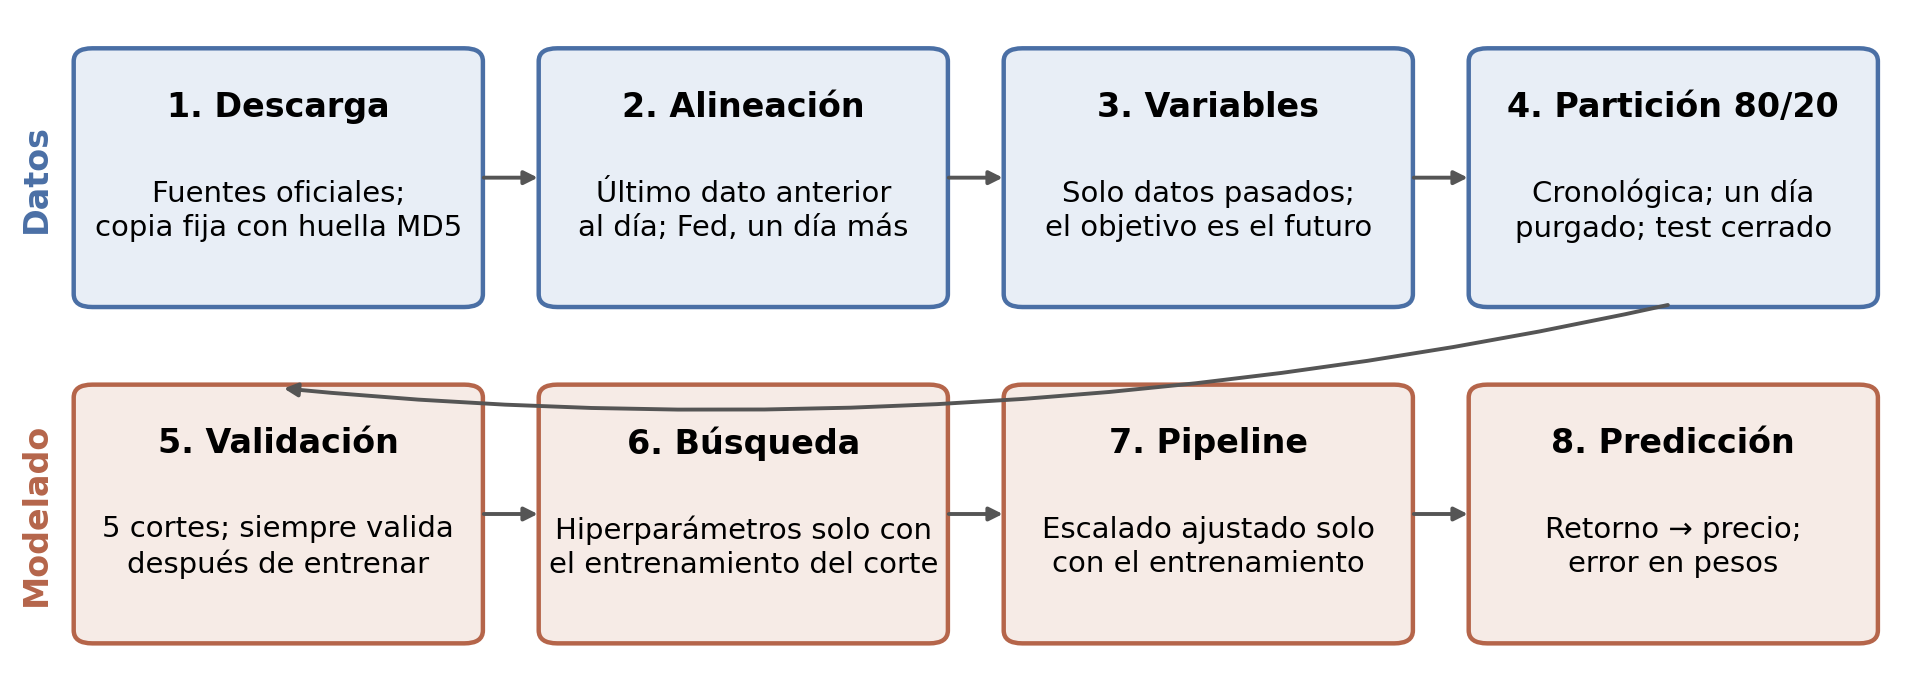
\includegraphics[width=0.8\textwidth]{fig_flujo.png}
\caption{Flujo del proyecto. Cada etapa usa solo información disponible en su momento.}
\label{fig:pipeline}
\end{figure}

Lo comprobamos así: una prueba automática detiene la ejecución si una variable usa un dato del mismo día o posterior, y alterar todos los datos posteriores a una fecha no cambia ninguna variable anterior. La partición es cronológica: 80~\% para desarrollo (2003 a marzo de 2022) y 20~\% para test (marzo de 2022 a 2026), con un día eliminado entre ambos porque su objetivo ya usa la TRM del test. De las transformaciones que lista la guía, solo el escalado de la regresión aprende de los datos, y va en un \texttt{Pipeline} con la búsqueda de hiperparámetros: solo aprende del entrenamiento de cada corte. No hay imputación (el relleno de festivos con el último dato solo mira al pasado), codificación (no hay categóricas), balanceo (es regresión) ni selección de variables con los datos (se fijaron en la Entrega~1). El análisis exploratorio y la elección del modelo usaron solo el desarrollo; el modelo elegido se congeló con huella MD5 y el test se abrió una sola vez. Con semilla fija, correr el proyecto desde cero reproduce todas las tablas exactamente.

% -------------------------------------------------------------------------------------
\section*{7.3. Reproducción y adaptación del método}

Primero aplicamos el método del artículo tal cual: precio en nivel, escalado MinMax ajustado con el entrenamiento, partición 80/20 y los tres algoritmos con su configuración por defecto. El artículo no dice qué variables usa, así que tomamos los rezagos 1, 5 y 10 de la Entrega~1, en nivel. Falla por una razón de fondo: un árbol predice promedios de lo que vio, así que nunca supera el máximo del entrenamiento. La Figura~\ref{fig:techo} lo muestra dentro del desarrollo: entrenando hasta julio de 2018, cuyo máximo fue 3.435 pesos, ninguna predicción pasó de 3.418 aunque la TRM superó los 4.100, y el error fue de 317 a 333 pesos. En el test se repite: la TRM llegó a 5.061, ninguna predicción pasó de 4.100 y el error fue de 295 a 306 pesos. La regresión lineal sí sigue a la TRM porque aprendió a copiar el valor de hoy (coeficiente de 1,02): error de 28 pesos y $R^2$ en nivel de 0,99, pero de 0,002 sobre retornos; no anticipa ningún movimiento.

\begin{figure}[!htbp]
\centering
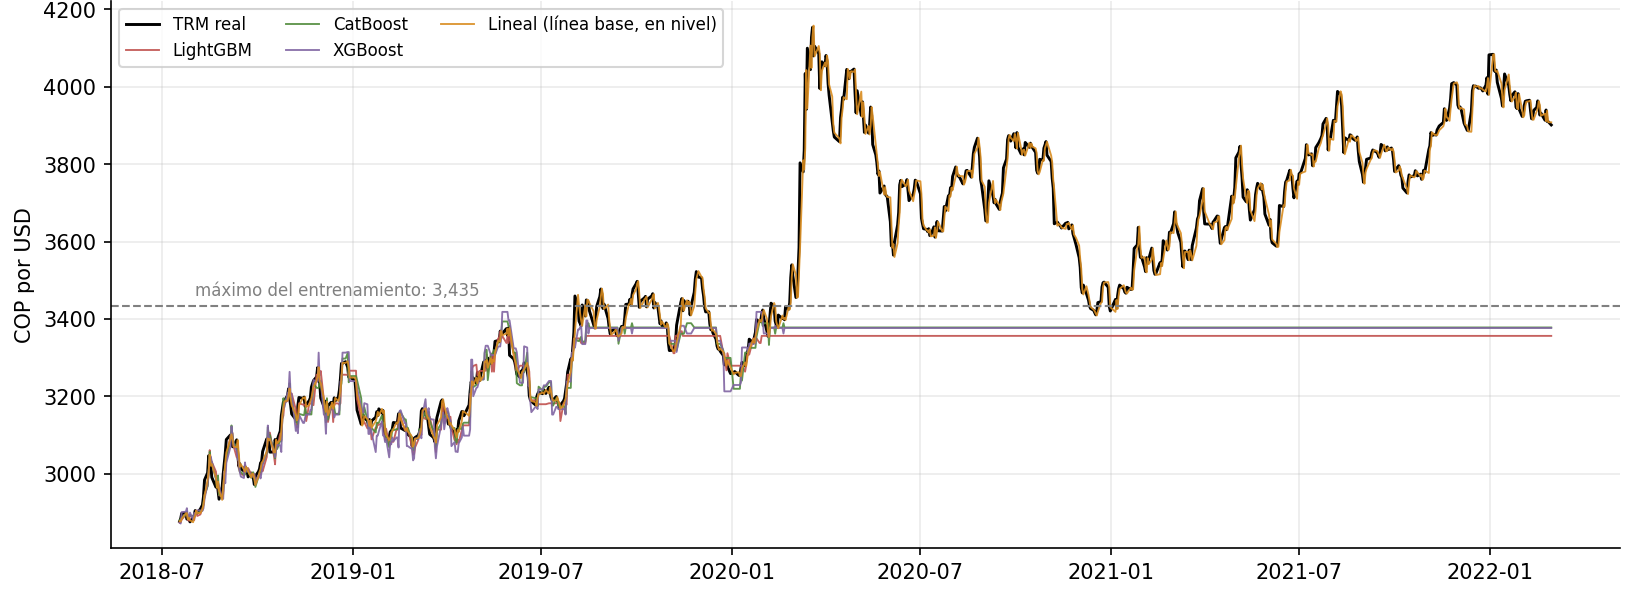
\includegraphics[width=0.66\textwidth]{fig03_techo_extrapolacion.png}
\caption{Método del artículo dentro del desarrollo (entrenamiento hasta julio de 2018, evaluación hasta marzo de 2022): las predicciones de los árboles se detienen en el máximo del entrenamiento.}
\label{fig:techo}
\end{figure}

La adaptación conserva lo que define al artículo: los tres algoritmos, el horizonte diario y la pregunta de cuál rinde mejor. La Tabla~\ref{tab:adaptacion} resume qué cambiamos y por qué. Frente a la Entrega~1 solo cambian el objetivo, el $R^2$, el petróleo (solo Brent), la alineación y la comparación con y sin macro.

\begin{table}[!htbp]
\centering\footnotesize
\setlength{\tabcolsep}{4pt}
\renewcommand{\arraystretch}{0.95}
\caption{Adaptación del método: qué hace el artículo, qué hacemos y por qué.}
\label{tab:adaptacion}
\begin{tabular}{l>{\raggedright\arraybackslash}p{3.3cm}>{\raggedright\arraybackslash}p{4.5cm}>{\raggedright\arraybackslash}p{4.9cm}}
\toprule
Elemento & Artículo & Nuestra adaptación & Por qué \\
\midrule
Datos & Cinco pares de divisas desarrolladas & TRM, Brent, DXY y diferencial Banrep--Fed & Contexto local: dólares del petróleo; tasa ligada a la Fed \\
Objetivo & Precio en nivel & Retorno del día siguiente & Los árboles no extrapolan en nivel (Figura~\ref{fig:techo}) \\
Variables & No las especifica & Las de la Entrega~1 en cambios diarios; solo Brent & Coherencia con el objetivo; WTI negativo en 2020 \\
Alineación & No aplica (una serie) & Último dato anterior al día; Fed, un día más & Cada dato entra cuando realmente se conoce \\
Validación & Un corte 80/20 & Cronológica y anidada (5 cortes) & Medir sin fuga y con variabilidad \\
Hiperparámetros & Por defecto & Búsqueda con validación cruzada temporal & Ajustarse a una señal débil \\
Comparación & Los tres entre sí & Con y sin macro, y frente a una línea base & Separar el algoritmo de las variables \\
Métricas & RMSE, MAE y $R^2$ en nivel & Las mismas; $R^2$ sobre retornos & En nivel no distingue de copiar la TRM \\
\bottomrule
\end{tabular}
\end{table}

\paragraph{Nuestros modelos.} La línea base es una regresión lineal sobre el movimiento de la TRM de hace 1, 5 y 10 días. Cada boosting se entrena con \emph{solo TRM}, las mismas tres variables, y con \emph{TRM + macro}, que agrega Brent, DXY y diferencial: seis configuraciones más la base. Con solo TRM, el boosting compite con la base con la misma información, así que si gana, el mérito es del algoritmo; la diferencia entre sus dos versiones mide el aporte macro.

\paragraph{Ajuste de hiperparámetros.} La Tabla~\ref{tab:hiper} muestra qué se ajusta, qué controla cada hiperparámetro, los valores posibles y los elegidos. Con scikit-learn \cite{sklearn} se toman al azar 15 combinaciones (semilla 42); cada una se evalúa con validación cruzada temporal de tres cortes, siempre validando con datos posteriores y con cinco días de separación, y gana la de menor error cuadrático. Los rangos favorecen modelos simples, porque la señal es débil y pocos días extremos podrían dominar el ajuste. Los modelos lo confirman: cinco de seis eligieron profundidad 2, todos una tasa de 0,05 o menos y entre 100 y 400 árboles. El ajuste se repite dentro de cada corte de la validación (7.4) y, al final, con todo el desarrollo para los modelos que van al test.

\begin{table}[!htbp]
\centering\footnotesize
\setlength{\tabcolsep}{3.5pt}
\caption{Hiperparámetros: qué controlan, valores posibles y valores elegidos en los modelos finales. Fijos: semilla 42, un hilo de cómputo y, en CatBoost, muestreo Bernoulli. La línea base no tiene hiperparámetros.}
\label{tab:hiper}
\resizebox{\textwidth}{!}{\begin{tabular}{l >{\raggedright\arraybackslash}p{5.6cm} >{\raggedright\arraybackslash}p{5.4cm} cc cc cc}
\toprule
 & & & \multicolumn{2}{c}{LightGBM} & \multicolumn{2}{c}{CatBoost} & \multicolumn{2}{c}{XGBoost} \\
\cmidrule(lr){4-5}\cmidrule(lr){6-7}\cmidrule(lr){8-9}
Hiperparámetro & Qué controla & Valores posibles & solo & macro & solo & macro & solo & macro \\
\midrule
Número de árboles & Cuántas correcciones se suman & 100; 200; 400; 800 & 200 & 200 & 200 & 200 & 100 & 400 \\
Tasa de aprendizaje & Cuánto corrige cada árbol & 0,01; 0,03; 0,05; 0,1 & 0,03 & 0,03 & 0,03 & 0,03 & 0,05 & 0,01 \\
Profundidad & Cuántas variables se combinan en una regla & 2; 3; 4; 6 & 2 & 2 & 2 & 4 & 2 & 2 \\
Mínimo por hoja & Días mínimos para crear una regla & 20; 50; 100; 200 (XGBoost: peso 1; 5; 10; 20) & 100 & 200 & 50 & 100 & 20 & 10 \\
Hojas máximas & Tamaño del árbol (solo LightGBM) & 4; 8; 15; 31 & 4 & 31 & -- & -- & -- & -- \\
Filas por árbol & Fracción de días que ve cada árbol & 0,6; 0,8; 1 & 0,6 & 0,6 & 0,8 & 1 & 1 & 0,8 \\
Variables por árbol & Fracción de variables que ve cada árbol & 0,6; 0,8; 1 & 0,8 & 0,8 & 0,8 & 1 & 0,6 & 1 \\
Regularización L2 & Cuánto se encogen las predicciones & 0; 1; 5; 10 (CatBoost: 1; 3; 5; 10) & 1 & 1 & 3 & 3 & 1 & 0 \\
\bottomrule
\end{tabular}
}
\end{table}

\paragraph{Comparación.} La Tabla~\ref{tab:resultados} muestra un empate. En validación, CatBoost con solo TRM mejora a la base en 0,13 pesos y por eso es el modelo elegido; en el test, la base tiene el menor error (35,63 pesos) y CatBoost queda a 0,01. Las macro no ayudan a ningún algoritmo: en validación bajan el error de LightGBM en 4 de 5 cortes, aunque en promedio lo dejan igual (+0,008 pesos), el de CatBoost en 2 y el de XGBoost en 1; en el test empeoran a los tres. LightGBM es el que menos pierde: 0,11 pesos, frente a 0,54 de XGBoost y 0,67 de CatBoost.

\begin{table}[!htbp]
\centering\footnotesize
\setlength{\tabcolsep}{4pt}
\caption{Resultados en validación (media $\pm$ desviación en 5 cortes, ver 7.4) y en el test. RMSE y MAE en pesos; $R^2$ sobre retornos. Macro mejora: cortes en que la versión con macro tiene menor RMSE que la de solo TRM. $\Delta$RMSE: diferencia con la línea base en el test. En negrita, el mejor de cada bloque.}
\label{tab:resultados}
\resizebox{\textwidth}{!}{\begin{tabular}{llcccc|cccc}
\toprule
 & & \multicolumn{4}{c|}{Validación (desarrollo, 5 cortes)} & \multicolumn{4}{c}{Test (una sola vez)} \\
\cmidrule(lr){3-6}\cmidrule(lr){7-10}
Algoritmo & Variables & RMSE (media $\pm$ desv.) & $R^2$ & Gana a la base & Macro mejora & RMSE & MAE & $R^2$ & $\Delta$RMSE \\
\midrule
Línea base (lineal) & solo TRM & 20,83 $\pm$ 7,00 & 0,019 & -- & -- & \textbf{35,63} & 27,10 & 0,037 & -- \\
\addlinespace[2pt]
LightGBM & solo TRM & 20,77 $\pm$ 6,87 & 0,017 & 3 de 5 &  & 35,75 & 27,22 & 0,032 & +0,12 \\
 & TRM + macro & 20,77 $\pm$ 6,85 & 0,018 & 2 de 5 & 4 de 5 & 35,86 & 27,26 & 0,027 & +0,23 \\
\addlinespace[2pt]
CatBoost & solo TRM & \textbf{20,71} $\pm$ 6,86 & 0,025 & 4 de 5 &  & 35,64 & 27,09 & 0,037 & +0,01 \\
 & TRM + macro & 20,77 $\pm$ 6,79 & 0,018 & 2 de 5 & 2 de 5 & 36,31 & 27,81 & 0,001 & +0,68 \\
\addlinespace[2pt]
XGBoost & solo TRM & 20,81 $\pm$ 6,85 & 0,016 & 3 de 5 &  & 35,79 & 27,25 & 0,029 & +0,16 \\
 & TRM + macro & 20,94 $\pm$ 6,76 & $-$0,002 & 1 de 5 & 1 de 5 & 36,32 & 27,82 & $-$0,001 & +0,70 \\
\bottomrule
\end{tabular}
}
\end{table}

% -------------------------------------------------------------------------------------
\section*{7.4. Validación, métricas e interpretación preliminar}

\paragraph{Validación y métricas.} Usamos validación anidada: el desarrollo se divide en cinco cortes cronológicos que entrenan con todo lo anterior y validan en los tres años siguientes, y los hiperparámetros se eligen solo dentro del entrenamiento de cada corte. Así nunca se elige y se mide con los mismos datos, lo que daría un error optimista. El RMSE en pesos es la métrica principal porque castiga más los errores grandes, los más costosos para un importador; el MAE da el error típico de un día y el $R^2$, qué parte del movimiento diario se explica. El desbalance no aplica por ser regresión; su equivalente son los días extremos, por eso reportamos RMSE y MAE juntos.

\paragraph{Variabilidad.} La ventaja de 0,13 pesos de CatBoost no es una mejora real: el error de cualquier modelo cambia unos 7 pesos entre periodos según la volatilidad, y CatBoost gana a la base en 4 de 5 cortes, pero siempre por centavos. El test tiene más error porque 2022--2026 fue más volátil.

\begin{figure}[!htbp]
\centering
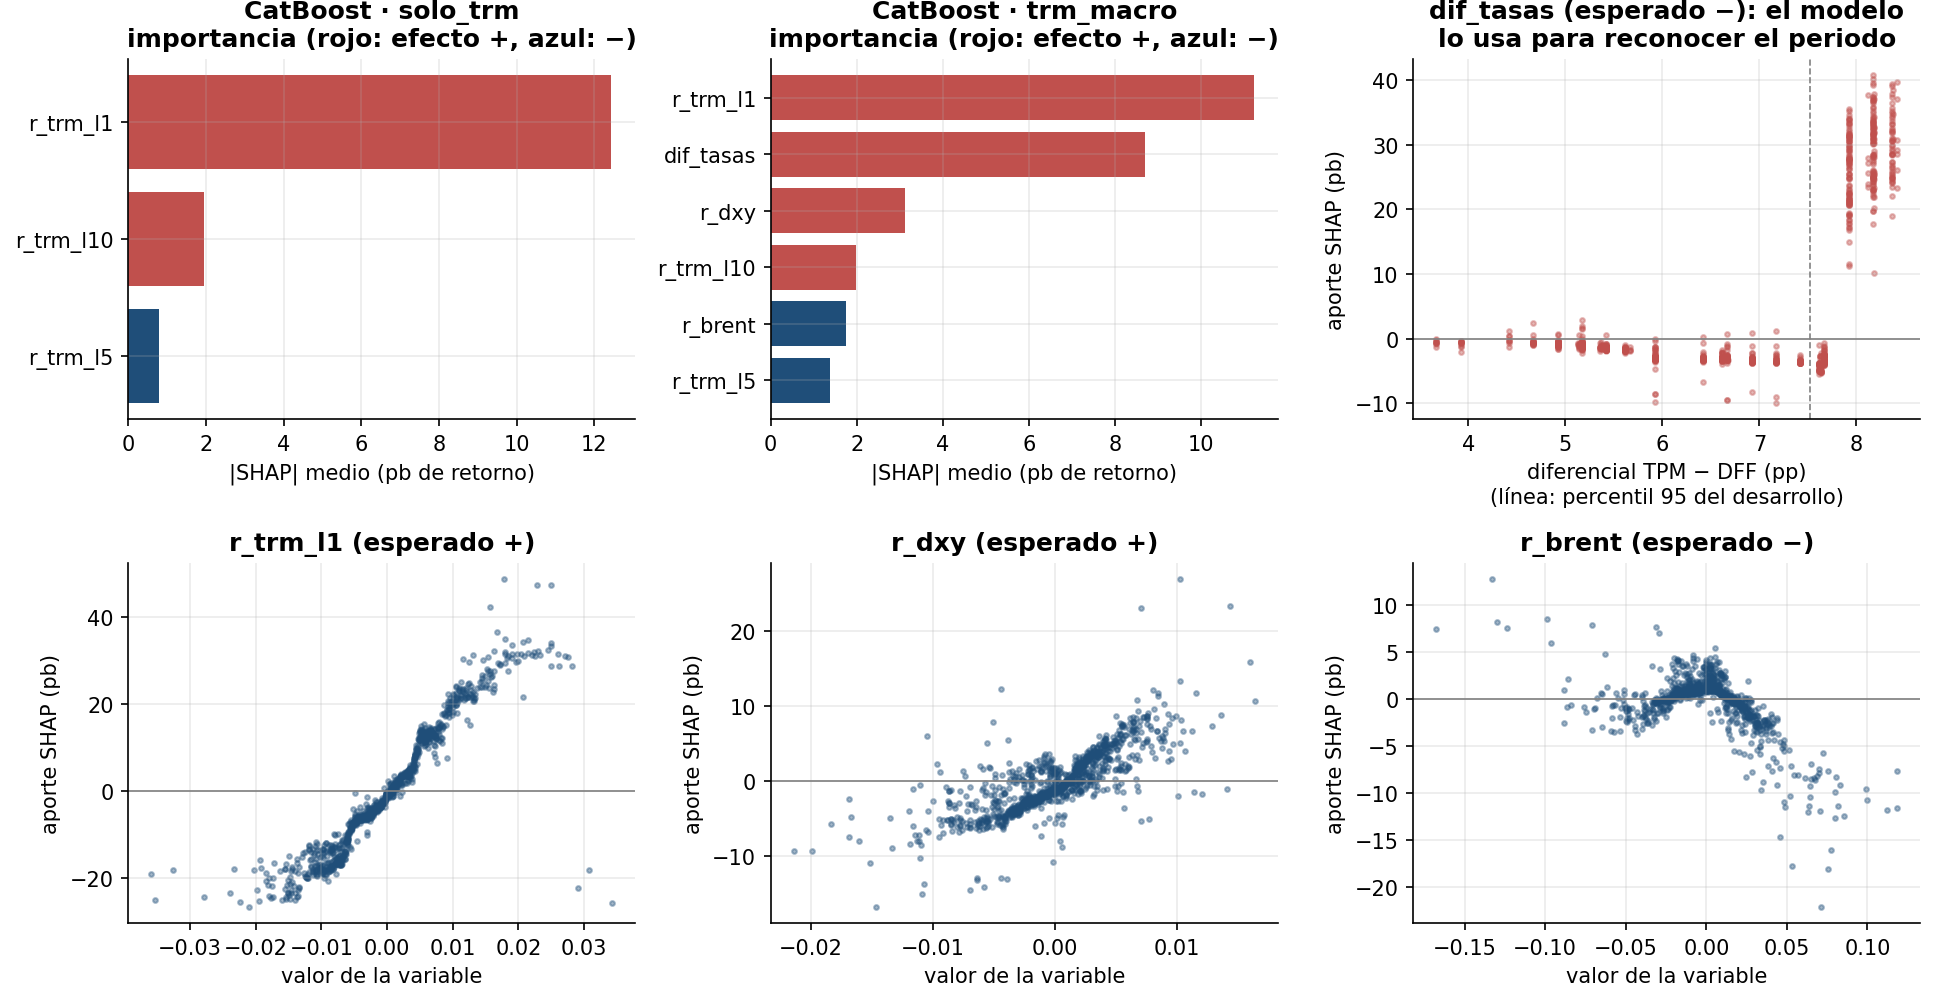
\includegraphics[width=0.64\textwidth]{fig05_shap.png}
\caption{Importancia de las variables (SHAP) en el test: CatBoost con solo TRM, CatBoost con macro y forma del efecto de cada variable.}
\label{fig:shap}
\end{figure}

\paragraph{Variables relevantes.} En el modelo elegido, el movimiento del día anterior concentra el 82~\% de la importancia y empuja la predicción en su dirección según SHAP \cite{shap} (Figura~\ref{fig:shap}). En la versión con macro, DXY y Brent actúan con el signo esperado, pero el diferencial de tasas toma el 31~\%: el modelo aprendió que un diferencial por encima de 7,8 puntos anuncia devaluación, porque en el desarrollo esos valores solo ocurrieron en devaluaciones. En el test fue alto durante una revaluación, y el modelo se equivocó de dirección. No es fuga de datos: es un cambio de régimen.

\paragraph{Estabilidad.} El resultado no depende del método de ajuste: repetir la validación con búsqueda bayesiana (Optuna \cite{optuna}), que aprende de los intentos anteriores, con 15 y 50 intentos, no cambia ningún error en más de 0,22 pesos (Tabla~\ref{tab:robustez}). Optuna es solo una prueba; los modelos finales son los de la búsqueda al azar. Sí cambia el orden de los modelos: la base pasa del sexto puesto en validación al primero en el test, algo esperable con diferencias menores que la variación entre periodos.

\begin{table}[!htbp]
\centering\footnotesize
\setlength{\tabcolsep}{4pt}
\caption{RMSE de validación (media de 5 cortes, en pesos) según el método de ajuste de hiperparámetros.}
\label{tab:robustez}
\begin{tabular}{l cc cc cc c}
\toprule
 & \multicolumn{2}{c}{LightGBM} & \multicolumn{2}{c}{CatBoost} & \multicolumn{2}{c}{XGBoost} & Línea \\
\cmidrule(lr){2-3}\cmidrule(lr){4-5}\cmidrule(lr){6-7}
Método de ajuste & solo & macro & solo & macro & solo & macro & base \\
\midrule
Al azar, 15 intentos (usado) & 20,77 & 20,77 & 20,71 & 20,77 & 20,81 & 20,94 & 20,83 \\
Optuna, 15 intentos & 20,76 & 20,78 & 20,71 & 20,68 & 20,73 & 20,72 &  \\
Optuna, 50 intentos & 20,76 & 20,76 & 20,70 & 20,70 & 20,74 & 20,81 &  \\
\midrule
Cambio máximo & 0,00 & 0,01 & 0,01 & 0,09 & 0,07 & 0,22 & -- \\
\bottomrule
\end{tabular}

\end{table}

\paragraph{Errores.} El error sigue a la volatilidad: el RMSE de la base fue de 46 pesos en la subida de 2022, 35 en la corrección siguiente y 28 en el choque petrolero de 2026. Todos fallan en los mismos días: los movimientos grandes no se anticipan con el dato de ayer. CatBoost con macro solo fue mejor en la subida de 2022, una devaluación como las que aprendió, y peor en las dos revaluaciones, lo que confirma la lectura de SHAP.

\paragraph{Implicaciones.} Para un importador, el mejor pronóstico de la TRM de mañana es la de hoy más el 17~\% de su movimiento (la línea base), con un error típico de 27 pesos; a un día, el boosting no justifica su complejidad. Es una conclusión preliminar: las diferencias son de centavos y vienen de un solo test. Para la entrega final queda tratar el cambio de régimen del diferencial.

% ===================== Final =====================
\clearpage
\begin{thebibliography}{99}
\small
\bibitem{articulo}
Eslami Ghayour, A., \& Yousefi, A. (2023). \textit{Performance Analysis of Gradient Boosting Models for Forex Market Prediction}. SSRN Preprint. \url{https://ssrn.com/abstract=4450688}

\bibitem{banrep}
Banco de la República de Colombia. \textit{Servicio web de estadísticas (SDMX): TRM y tasa de política monetaria}. \url{https://www.banrep.gov.co}

\bibitem{superfin}
Superintendencia Financiera de Colombia. \textit{Tasa de Cambio Representativa del Mercado}. Datos Abiertos Colombia. \url{https://www.datos.gov.co}

\bibitem{fred}
Federal Reserve Bank of St. Louis. \textit{Brent - Europe (DCOILBRENTEU) y Federal Funds Effective Rate (DFF)}. FRED. \url{https://fred.stlouisfed.org}

\bibitem{yahoo-dxy}
Yahoo Finance. \textit{US Dollar Index (DX-Y.NYB)}. \url{https://finance.yahoo.com/quote/DX-Y.NYB}

\bibitem{shap}
Lundberg, S. M., \& Lee, S.-I. (2017). A Unified Approach to Interpreting Model Predictions. \textit{Advances in Neural Information Processing Systems}, 30.
\bibitem{lightgbm}
Ke, G., et al. (2017). LightGBM: A Highly Efficient Gradient Boosting Decision Tree. \textit{Advances in Neural Information Processing Systems}, 30.

\bibitem{catboost}
Prokhorenkova, L., et al. (2018). CatBoost: Unbiased Boosting with Categorical Features. \textit{Advances in Neural Information Processing Systems}, 31.

\bibitem{xgboost}
Chen, T., \& Guestrin, C. (2016). XGBoost: A Scalable Tree Boosting System. \textit{Proceedings of the 22nd ACM SIGKDD Conference}, 785--794.

\bibitem{sklearn}
Pedregosa, F., et al. (2011). Scikit-learn: Machine Learning in Python. \textit{Journal of Machine Learning Research}, 12, 2825--2830.

\bibitem{optuna}
Akiba, T., et al. (2019). Optuna: A Next-generation Hyperparameter Optimization Framework. \textit{Proceedings of the 25th ACM SIGKDD Conference}, 2623--2631.
\end{thebibliography}

\paragraph{Código.} Repositorio del proyecto, carpeta \texttt{Entrega 2}; el README indica la instalación y el orden de ejecución:\\
\url{https://github.com/Gatitomalo1234/Proyecto-Machine-Learning-2}

\paragraph{Uso de IA.} Usamos Claude (Anthropic) como asistente para estructurar el código, revisar la metodología frente a la rúbrica y redactar borradores. Las decisiones y la interpretación son nuestras, y verificamos cada cifra contra las salidas del código.

\end{document}
